% !TEX TS-program = pdflatex
% !TEX encoding = UTF-8 Unicode

\documentclass[11pt]{article} % use larger type; default would be 10pt

\usepackage[utf8]{inputenc} % set input encoding (not needed with XeLaTeX)

%%% PAGE DIMENSIONS
\usepackage{geometry} % to change the page dimensions
\geometry{a4paper} % or letterpaper (US) or a5paper or....

\usepackage{graphicx} % support the \includegraphics command and options

%%% PACKAGES
\usepackage{booktabs} % for much better looking tables
\usepackage{array} % for better arrays (eg matrices) in maths
\usepackage{paralist} % very flexible & customisable lists (eg. enumerate/itemize, etc.)
\usepackage{verbatim} % adds environment for commenting out blocks of text & for better verbatim
\usepackage{subfig} % make it possible to include more than one captioned figure/table in a single float
\usepackage{amsmath}
\usepackage{hyperref}


%%\usepackage{dsfont}

%%% HEADERS & FOOTERS
\usepackage{fancyhdr} % This should be set AFTER setting up the page geometry
\pagestyle{fancy} % options: empty , plain , fancy
\renewcommand{\headrulewidth}{0pt} % customise the layout...
\lhead{}\chead{}\rhead{}
\lfoot{}\cfoot{\thepage}\rfoot{}


%%% SECTION TITLE APPEARANCE
\usepackage{sectsty}
\allsectionsfont{\sffamily\mdseries\upshape} % (See the fntguide.pdf for font help)
% (This matches ConTeXt defaults)

%%% ToC (table of contents) APPEARANCE
\usepackage[nottoc,notlof,notlot]{tocbibind} % Put the bibliography in the ToC
\usepackage[titles,subfigure]{tocloft} % Alter the style of the Table of Contents
\renewcommand{\cftsecfont}{\rmfamily\mdseries\upshape}
\renewcommand{\cftsecpagefont}{\rmfamily\mdseries\upshape} % No bold!



\newcommand{\euley}{U\sqrt{\Lambda}\eta}
\newcommand{\uley}[1]{\euley_#1}

%\graphicspath{{./pics}}
%%% END Article customizations

%%% The "real" document content comes below...

\title{CQF Final Project Report}
\author{Rustam Guseynov}
%\date{} % Activate to display a given date or no date (if empty),
         % otherwise the current date is printed 

\begin{document}
\maketitle
\begin{abstract}
When I implemented this project, my primary goal was to better understand the models and find answers to questions I couldn't answer before. Hence, I tried to avoid reproducing all formulas already provided and proven in textbooks or going into great details of well-known mathematical methods I used. At the same time I try to show which choice I had during project implementations, what decisions I made, and why.
\end{abstract}

%% ---> INTRO <--- %% 
\section{Introduction}
\subsection{Computational environment}
I have chosen Matlab as a primary programming environment. The choice was determined by the unique features of Matlab: easy vector operations, lots of built-in linear algebra algorithms, and convenience of programming language itself. It supports advanced programming techniques like anonymous functions and structures with dynamic fields. It also supports OOP and code structuring via packages. Matlab allows to concentrate on the task first, and then go to details as deep as it's necessary.

Matlab also has a very convenient feature of storing data in its native ``.mat'' files, which were like Excel spreadsheets or database tables. I have once downloaded, structured and imported source data, and then stored them into .mat file, which is reloaded each time script runs.

My code can be also run with Octave.
\subsection{Choice of assignments}
After thorough examination of the options available, I have chosen HJM Model and Static Hedge. The reason for HJM Model was to obtain hands-on experience with interest rate models, which I find essential to understand quantitative finance. Interest rate models are more complex than equity model because of incompleteness of interest rate market, and at the same time, they are good starting point for more advanced models, for example, credit risk models.

Static Hedge is was chosen for two reasons: first, I did FDM when studied in university, and second is that uncertain parameters models look very impressive because they are simple and they solve very advanced problems. Uncertain parameters approach can easily incorporate uncertain interest rate and uncertain dividends, which together with uncertain volatility covers most substantial uncertainties in pricing of contingent claims. Static hedging in this setting is essential to narrow bid-ask spread on securities, priced with uncertain parameters model.

\section{HJM Model}

%% === Some bad words about short-rate models === %%
\subsection{Comparing to short-rate models}

HJM model was the first interest rate model which took advantage of modelling whole yield curve instead of modelling only one point of that curve like it was in short-rate models.

Why do I say ``advantage''? Generally speaking, there's nothing wrong with short-rate models, but there's something unnatural in the way they treat bond pricing and yield curve modelling. Here's what I mean.\\
Let's take spot yield curve r(t). Instantaneous forward yield curve is then % TODO REFERENCE
\begin{equation}
f(t) = \frac{d}{dt}(rt) = r(t) + r'(t) t
\end{equation}
and, conversely, 
\begin{equation}
r(t) = \frac{1}{t}\int_{0}^{t}{f(s)ds}
\end{equation}
Price of zero-coupon bond is computed very naturally, by discounting bond future (face) value by rate, corresponding to the term of the bond:
\begin{equation} \label{eq:truebondprice}
Z(0,T) = e^{-r(T)T} = exp\left(-T\frac{1}{T}\int_{0}^{T}{f(s)ds}\right) = exp\left(-\int_{0}^{T}{f(s)ds}\right)
\end{equation}

These formulas are very intuitive and could be used directly should we have behaviour of spot or forward yield curve modelled. But in case of short-rate models what we model is short rate $r(0) = r_0$ and thus it is impossible to get $r(T)$ directly. Without understanding of yield curve movements, one has to consider ZCB to be a derivative on short rate and look for solution of bond pricing equation (Black-Scholes equation for bond) in form 
\begin{equation} 
Z(t,T) = e^{A(t,T) r + B(t,T)}
\end{equation}
Comparing this equation to ``true'' bond pricing formula \eqref{eq:truebondprice}, I conclude that short-rate models approximate longer interest rate with linear function of $r_0$ in form $A(t,T) r_0 + B(t,T)$. One could call it a ``first-order approximation''. Later on one could estimate full yield curve $r(t,T)$ and forward curve $f(t,T)$ from these bond prices
\begin{alignat}{2}
r(t,T) = -\frac{\ln Z(t,T)}{T-t},\\
\label{eq:fwdfrombond} f(t,T) = -\frac{d \ln Z(t,T)}{dT}
\end{alignat}
Thus short rate models are a ``double trouble'': a headache to implement and deduce bond prices, and only a first-order approximation of true dynamics of yield curve.\\

%% === Basic ideas behind HJM === %%
\subsection{HJM setting}

As I have already told before, HJM is a model of a whole yield curve. Or, more specifically, of an instantaneous forward yield curve.\\

\cite[ch. 37]{PWoQF06} starts with premise that ZCB price follows some general lognormal random walk
\begin{alignat}{1} \label{eq:lognrmal_bond}
dZ(t,T) = \mu(t,T)Z(t,T)dt + \sigma(t,T)Z(t,T)dW_{t}\\
\forall t \text{ } Z(t,t) = 1 \nonumber
\end{alignat}
Integrating  \eqref{eq:lognrmal_bond} into 
\begin{equation}
lnZ(t,T) = \left(\mu(t,T)-  \frac{1}{2}\sigma^2(t,T)\right)t +\sigma(t,T)W_{t}
\end{equation}
and substituting into \eqref{eq:fwdfrombond} he obtains
\begin{equation}
f(t,T) = \frac{\partial}{\partial T}\left(\frac{1}{2}\sigma ^2(t,T) - \mu(t,T)\right) t-\frac{\partial}{\partial T}\sigma(t,T)W_{t}
\end{equation}
It can be shown (\cite[par. 10.3.2]{Shreve08} for example) that in risk-free case $\mu(t,T) = r(t)$. Thus 
\begin{equation}
f(t,T) = \sigma(t,T)\frac{\partial \sigma(t,T)}{\partial T}t-\frac{\partial}{\partial T}\sigma(t,T)W_{t}
\end{equation}
Introducing $\nu(t,T) = -\frac{\partial}{\partial T}\sigma(t,T)$ and differentiating we obtain almost final version of forward rate SDE
\begin{equation}
df(t,T) = \nu(t,T)\left(\int_{t}^{T}\nu(t,s)ds\right)dt + \nu(t,T)dW_{t} \nonumber
\end{equation} 

Finally, applying Musiela parametrization $\nu(t,T) = \bar{\nu}(t,T-t)$ and SDE becomes
\begin{equation} \label{eq:hjm_musiela}
d\bar{f}(t,\tau) = \left[\bar{\nu}(t,\tau)\int_{0}^{\tau}\bar{\nu}(t,s)ds+ \frac{\partial}{\partial \tau}\bar{f}(t,\tau)\right]dt + \bar{\nu}(t,\tau)dW_{t} 
\end{equation}
where $\tau = T-t$.

%% === How to discretize === %%
\subsection{Dimensionality and dimension reduction}
The main input into equation \eqref{eq:hjm_musiela} is $\bar{\nu}(t,\tau)$. In this model we do not simulate or forecast volatility, hence we use constant volatility model. This means that $\bar{\nu}(t,\tau) = \nu(\tau)$, which is known at time zero. That volatility function is an only source of randomness in SDE. Term $\bar{\nu}(t,\tau)dW_t$ means that on each step the whole yield curve will experience a shift proportional to value of $\bar{\nu}(t,\tau)$ at particular term $\tau$. At the same time the model can easily be extended so that to introduce several random walks. It takes form
\begin{alignat}{1} \label{eq:hjm_musiela_multidim}
d\bar{f}(t,\tau) = \left[\sum_{k=1}^N\bar{\nu_k}(\tau)\int_{0}^{\tau}\bar{\nu_k}(s)ds+ \frac{\partial}{\partial \tau}\bar{f}(t,\tau)\right]dt + \sum_{k=1}^N\bar{\nu_k}(\tau)dW_{t, k}\\
\forall k = \overline{1:N} \nonumber
\end{alignat}
where $N$ is number of components.

We calibrate the model to the historical data, so we can easily estimate interest rates covariance matrix $\Omega$. Let us suppose we have history on $N$ interest rates of different terms. In this case covariation matrix components are determined by $(\Omega)_{ij} = \rho_{ij}\sigma_{i}\sigma_{j}$ and $\Omega \in R^{N \times N}$, where $\rho_{ij} = corr(r_i,r_j)$ - correlation of $i^{th}$ and $j^{th}$ interest rates and $\sigma_i$ is standard deviation of $i^{th}$ rate.

In this case we have simulate N correlated random walks. In appendix~\ref{ap:PCA} it is shown that there's an easy way to reduce number of random walks by extracting principal components.

%% === How to simulate === %%

\subsection{Implementation}
\subsubsection{Data}
I use two datasets. First is Bank of England yield curves, as suggested in project description and another is a set of MICEX \footnote{Major Russian exchange} OFZ\footnote{Russian domestic treasury bonds} curves. 
Both datasets are stored in Matlab files: hjm\_boe\_forward.mat and hjm\_micex\_nss.mat.
Bank of England yield curves are ready to use, and after loading hjm\_boe\_forward.mat file I obtain main variables: terms (1D array of terms of interest rates) and rates(2D array of interest rates history). 

MICEX data are a bit more contrived. The data consists of a list of daily parameters of extended Nelson-Siegel-Svennson\footnote{More detailed description is available on MICEX \href{http://rts.micex.ru/a80}{website}} approximation of validated and bootstrapped OFZ curves. I store this list in hjm\_micex\_nss.mat. After loading it I create my own grid of terms and evaluate rate curves at these points. Then I recalculate them into forward rates.

Choice between data sources depends on SELECTED\_MODEL variable. It can take two values, BANK\_ENGLAND\_FWD and MICEX\_NSS.

\subsubsection{Discretization}
In order to simulate equation \eqref{eq:hjm_musiela_multidim}, we have to replace it with its discrete version. First I will discretize it by $t$. Time $t$ starts at zero and has step of arbitrary fixed length $\delta t$.
\begin{equation}
\bar{f}_i(\tau) - \bar{f}_{i-1}(\tau) = \left[\sum_{k=1}^N\bar{\nu_k}(\tau)\int_{0}^{\tau}\bar{\nu_k}(s)ds+ \frac{\partial}{\partial \tau}\bar{f}_{i-1}(\tau)\right]\delta t + \sum_{k=1}^N\bar{\nu_k}(\tau)\delta W_{k}
\end{equation}
Here $N$ is number of principal components, and $i$ ranges from $1$ to artbitrary chosen period of time.

Next step is discretization by terms $\tau$. In my case it is either done exogenously (Bank of England data are already discretized by the Bank by terms) or I could do it myself. This means I have a system of $M$ equations, there $M$ is number of points on term grid.
\begin{equation} \label{eq:hjm_musiela_multidim_discrete}
\bar{f}_i^j - \bar{f}_{i-1}^j = \left[\sum_{k=1}^N\bar{\nu_k}(\tau_j)\int_{0}^{\tau_j}\bar{\nu_k}(s)ds+ \frac{\bar{f}_{i-1}^j-\bar{f}_{i-1}^{j-1}}{\delta\tau_j}\right]\delta t + \sum_{k=1}^N\bar{\nu_k}(\tau_j)\delta W_{k}
\end{equation}
where $j = \overline{1:M}$ and $\delta\tau_j = \tau_j - \tau_{j-1}$ is a length of $j^{th}$ term grid step. 

The only undiscretized thing here is integral $\int_{0}^{\tau_j}\bar{\nu_k}(s)ds$. $\bar{\nu}(\tau)$ is a function with known values on grid points. Hence we can easily do a numerical integration using, for example, standard trapezoid rule:
\begin{equation}
\int_{0}^{\tau_j}\bar{\nu_k}(s)ds = \sum_{i=1}^{j-1}\frac{\bar{\nu_k(\tau_i)}+\bar{\nu_k(\tau_{i+1})}}{2}\delta\tau_i
\end{equation}

Another approach is to use approximated principal components. In this case integration is performed as described in appendix~\ref{ap:Polynom}

\subsubsection{Volatility structure}
The last issue I wanted to discuss is volatility structure. In \cite[par. 37.15]{PWoQF06} it is told that standard HJM model might give negative interest rates. That was exactly what I have gotten, and it was a bit irritating. 

To avoid it I implemented a non-infinitesimal short rate model as it is explained in there. In order to switch from standard to non-infinitesimal model it is necessary to set variable LOGNORMAL from $0$ to $1$.

One thing left unclear for me was if it is correct to use same principal components (e.g. same covariance matrix)? In non-infinitesimal model we work with m times compounded interest rates. In this case it might be correct to recalculate our interest rates into corresponding compounding and calculate covariance matrix for such rates. Recalculation is done using formula $r_m = m\left((1+r_1)^{1/m}-1\right)$. There's significant difference in principal components:\\
 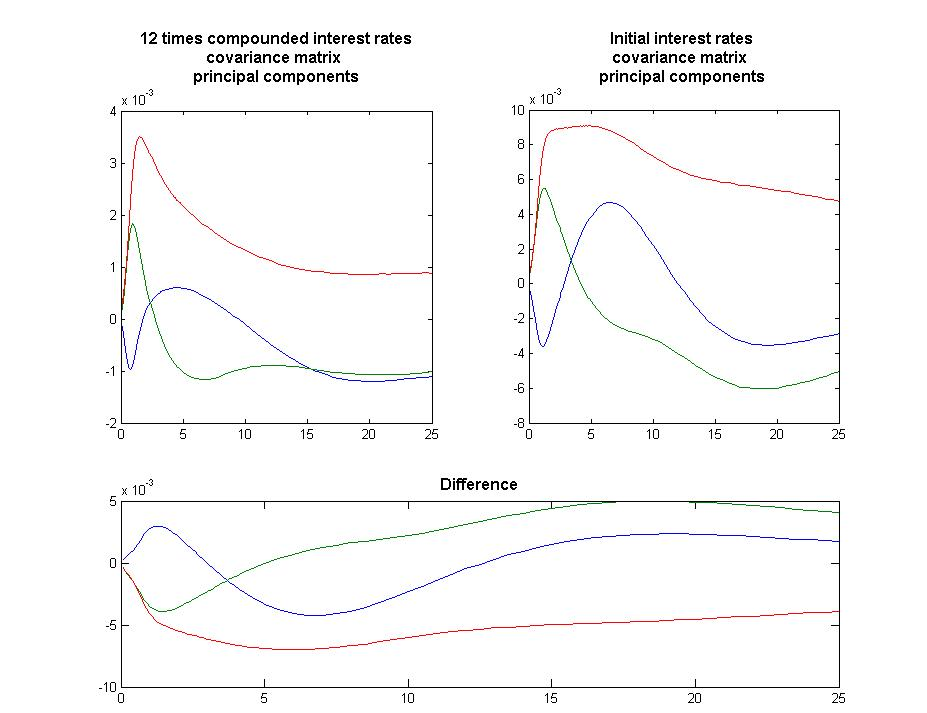
\includegraphics[scale=0.4]{compounding_PCA.jpg}\\
In this case no negative interest rates occur.

\subsubsection{Fitting eigenvectors with polynomials}


\subsubsection{Volatility structure}
\subsection{Pricing financial instruments}
\subsubsection{Zero-coupon bond}
\subsubsection{Cap pricing}

\subsection{Other models}

\subsection{Further improvements}


%% ---> STATIC HEDGE <--- %%
\section{Uncertain volatility and static hedge}
\subsection{Task description}
Uncertain volatility model assumes volatility to be not just random, but uncertain, i.e. we do not know anything about its distribution and can rely only on its expected range. Contingent claim price is still determined by Black-Scholes equation, but instead of constant volatility this equation now uses the most undesirable variable of volatility from that range. This means that instead of constant $\sigma$ equation contains $\sigma = \sigma(\Gamma)$, which definition depends on whether option is long or short. For more details I refer to \cite[ch. 52 and 60]{PWoQF06}.

So the task basically consist of two major parts. First is to solve non-linear bond pricing equation (as described above) and the second is to solve optimization problem. The goal of the second part is to find combination of our option being priced with other traded instruments, which (combination) will have least residual cost. 

Optimization doesn't make sense for linear pricing models, because in linear pack of options cost is exactly the same as the sum of their prices. That's not the case for non-linear models. One can create a pack, which will contain some non-traded exotic option and number of traded vanilla options. Then he or she will try to solve optimization problem: $[\lambda_1, ..., \lambda_N] = \underset{[\lambda_1, ..., \lambda_N]\in \mathbf{R}^N}{\arg \min} \left[\text{Price}\left(\text{Exotic} + \sum_{i=1}^{N}\lambda_i \text{Vanilla}_i\right) - \sum_{i=1}^N\lambda_i\text{Price}\left(\text{Vanilla}_i\right) \right]$.

Application of static hedge allows to narrow bid-ask spread on exotic product, which price is calculated using uncertain parameters model.

\subsection{Pricing}
Price of derivatives in question can be found as a solution of Black-Scholes PDE, which takes form of:
\begin{equation}
\frac{\partial V}{\partial t} + \frac{1}{2}\sigma^2 S^2 \frac{\partial^2 V}{\partial S^2} +rS\frac{\partial V}{\partial S} - rV = 0
\end{equation}
Discretization of this equation requires us to introduce grids on time and asset price axes. If time $t \in [0,T]$, then grid $\omega_t$ is $\omega_t = \lbrace t_k = k\delta t, k = 0...N_t-1, \delta t = T/N_t\rbrace$. $N_t$ is arbitrary chosen number of points on time axis. Similarly, asset price grid is $\omega_S = \lbrace S_i = i\delta s, i = 0...N_s-1, \delta s = S_{max}/N_s\rbrace$.\\

I will use the following symbols for difference operations:
\begin{itemize}
	\item Right first-order derivative: $V_x =\frac{V_{i+1}-V_i}{h}$
	\item Left first-order derivative: $V_{\overline{x}} =\frac{V_{i}-V_{i-1}}{h}$
	\item Central first-order derivative: $V_{\mathring{x}} =\frac{V_{i+1}-V_{i-1}}{2h}$
	\item Second order derivative $V_{x\overline{x}} = \left(\frac{V_{i+1}-V_i}{h} - \frac{V_{i}-V_{i-1}}{h}\right)/h = \frac{V_{i+1}-2V_{i}+V_{i-1}}{h^2}$
\end{itemize}
Finite difference approximation of BS equation at point $(i,k)$ is the following:
\begin{equation}
V_t + \sigma^2 S_i^2 V_{\overline{x}x} + r S_i V_{\mathring{x}} + rV_i = 0
\end{equation}
If last three terms of previous equation are taken at time step $k$, the scheme is explicit, and when $k+1$ is used, the scheme is implicit.

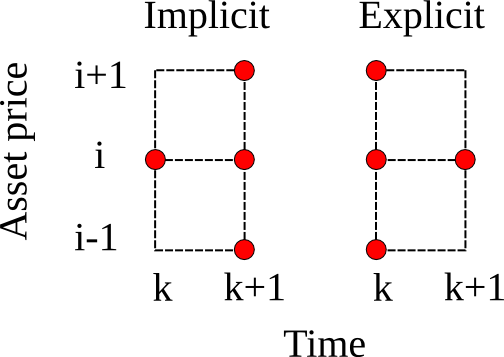
\includegraphics[scale=0.5]{schemes.png}\\ 

\subsection{Optimization}
It is a part of 


\subsection{Finite-difference method}
Finite difference methods approach suggest substitution of partial derivatives with their approximation with finite differences. The problem that arises is accuracy of such approximation and its convergence.

\subsection{Optimization}

\subsection{Results}
\subsection{Further improvements}
 - American options\\
 - Barrier options\\
 - Uncertain interest rate\\
 - Better schemes with improved convergence\\
 - Irregular grids
 
%% ---> APPENDICES <--- %%
\appendix

%% === Principal component analysis === %%
\section{PCA and simulation of correlated random walks}
\label{ap:PCA}

Any matrix is simply a linear transformation in multidimensional vector space. It is well known that any matrix can be decomposed into set of rotations, shifts and scalings. \\

Let us suppose we have a covariance matrix $\Omega \in R^{N \times N}$ and vector of i.i.d. standard normal random variables $\eta \in R^N$. It is known that for any covariance matrix there exist self-adjoint matrices $U, \Lambda \in R^{N \times N}$ where $U$ contains columns of eigenvectors and $\Lambda \text{ = } diag(\lambda_1, ..., \lambda_N)$ - eigenvalues of matrix $\Omega$. The eigenvalues are non-negative due to nature of covariance matrix.


\subsection{Generating correlated random walks using eigenvalcommunityue decomposition}
I will start with vector $\eta = (\eta_1, ..., \eta_N)$ of i.i.d standard normal random variables. My goal is to obtain vector $\xi$ of correlated standard normal random variables. Desired correlation structure is described by covariance matrix $\Omega$.

Eigenvalue decomposition of covariance matrix is $\Omega = U \Lambda U^T = \left(U\sqrt{\Lambda}\right) \left(U\sqrt{\Lambda}\right)^T$. Let $\xi =\euley$. In such case

\begin{equation}
cov(\xi_i,\xi_j) = 
E\left[(\xi_i-E\xi_i)(\xi_j-E\xi_j)\right] =
E\left[\left(\uley{i}-E\uley{i}\right)\left(\uley{j}-E\uley{j}\right)\right]  \nonumber 
\end{equation}
Taking into account that $E\uley{i} = 0 \text{ for any } i$ we obtain
\begin{multline}
E\left[\left(\sum{u_{ik}\sqrt{\lambda_k}\eta_k}\right)\left(\sum{u_{jk}\sqrt{\lambda_k}\eta_k}\right)\right] = \\
E\sum{u_{ik}\sqrt{\lambda_k}\eta_k u_{jm}\sqrt{\lambda_m}\eta_m} = \\
\sum{u_{ik}\sqrt{\lambda_k}u_{jm}\sqrt{\lambda_m}E(\eta_k\eta_m)} = \\
 \{\eta\text{`s are standard normal i.i.d}\} = \\
\sum{u_{ik}\lambda_ku_{jk}} = \left(\Omega\right)_{ij} \text{, q.e.d}
\end{multline}

\subsection{Reducing number of dimensions}
Now vector $\xi$ can be written as  $\xi = \sum{U_k\sqrt{\lambda_k}\eta_k}$, where $U_k$ is $k^{th}$ eigenvector. Evidently, $\xi$ is a sum of vectors $\eta$ weighted by their eigenvalues. This means we can select only $K$ largest eigenvalues for which value
\begin{equation}
R = \frac{\sum_{i=1}^K{\sqrt{\lambda_i}}}{\sum_{i=1}^N{\sqrt{\lambda_i}}}
\end{equation} 
is greater than some threshold (for example, 95\%).

%% === Polynomial approximation === %%
\section{Polynomial approximation}
\label{ap:Polynom}

In order to generate smooth and nicely correlated trajectories of interest rates of adjacent terms, we have to smooth the eigenvectors obtained by PCA as described in appendix~\ref{ap:PCA}. These vector already look smooth, but polynomial approximation has an advantage that it allows easy iteration and differentiation without using any numerical procedures. 
\subsection{Polynomial function representation}
Suppose we have a polynomial $P_N(t) = \sum_{k=0}^N a_k t^k$ of power $N$. Then it can be stored as a vector of its $N+1$ components $V_{N+1} = [a_0, a_1, ..., a_N]$.

Integration of this polynomial on range from $0$ to arbitrary value $t$ would give $\int_0^t{P_N(s)ds} = P_{N+1}(t) = \sum_{k=0}^{N} \frac{a_k}{k+1} t^{k+1}$
which in vector representation is $V_{N+2} = \left[0, \frac{a_0}{1}, \frac{a_1}{2}, ..., \frac{a_N}{N+1}\right]$. 

Similarly, differentiation would give $\frac{dP_N(t)}{dt} = P_{N-1}(t) = \sum_{k=1}^{N-1} ka_k t^k$ which in vector representation is $V_{N} = \left[a_1, 2a_2 ..., Na_N\right]$.

\subsection{Solving for polynomial parameters}
Now, how should one obtain polynomial approximation of arbitrary function given its values on some grid? 

Suppose that we have an interval $x \in [A,B]$ which is divided into not necessarily even parts $A = x_0, x_1, ..., x_{N-1}, x_N = B$ and we have values $y_i = y(x_i) \text{ for } x = \overline{0:N}$. We want to find the closest approximation of that grid function $y_i$ with polynomials of degree of $N$ in mean-square sense. 

This means we have to solve optimization problem 
\begin{equation}
J(\theta) = \frac{1}{N+1}\sum_{k=0}^{N}\left(y_k-f(\theta,x_k)\right)^2 \to max
\end{equation} where $f(\theta_N,x) =  \sum_{k=0}^N \theta_k x^k$.
Using vector notation. we can rewire it as follows:
\begin{equation}
\theta = argmax\left[J(\theta) = \left(\mathbf{y}-\mathbf{\theta \cdot x}\right)^T\left(\mathbf{y}-\mathbf{\theta \cdot x}\right)\right]
\end{equation} 
Here $y = (y_1, ..., y_N)^T$, $\theta = (\theta_1,...\theta_M)$ and 

\begin{equation}
X = 
\begin{pmatrix}
1 & x_1 & \cdots & x_1^M \\
1 & x_2 & \cdots & x_2^M \\
\vdots & \vdots & \cdots & \vdots \\
1 & x_N & \cdots & x_N^M 
\end{pmatrix}
\nonumber
\end{equation} 

Using rules of \href{http://en.wikipedia.org/wiki/Matrix\_calculus}{matrix calculus} we can solve this optimization problem by solving equation 
\begin{alignat}{1}
\frac{dJ(\theta)}{d\theta} = 0 \iff 
\frac{d}{d\theta} \left(\mathbf{y}-\mathbf{X\theta}\right)^T\left(\mathbf{y}-\mathbf{X\theta}\right) = 0
\iff \nonumber \\
\mathbf{X^T}(\mathbf{y-X\theta}) = 0 \iff \theta = \mathbf{\left(X^T X\right)^{-1}X^T y}
\end{alignat}
The latter is a so-called ``normal equation''. It is very convenient to use allowing to obtain solution in one step. This contrasts to iterative methods of solving optimization problem, where you would need to normalize independent variables, calculate gradient of cost function $J(\theta)$ and searching for optimal step size. 

Example of approximation of eigenvectors with $3^{rd}$ order polynomials below:\\
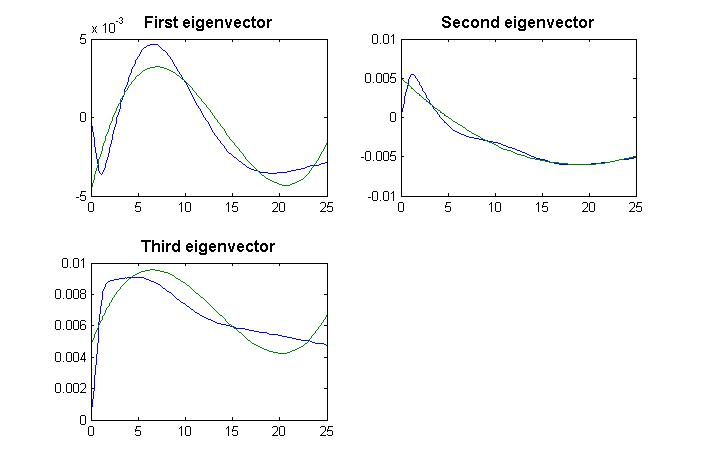
\includegraphics[scale=0.6]{fitting.jpg}\\

%% ---> BIBLIOGRAPHY <--- %%
\begin{thebibliography}{9}
\bibitem{PWoQF06} Paul Wilmott, \emph{Paul Wilmott on Quantitative Finance}, 2nd Edition, 2006.
\bibitem{Shreve08} Steven E. Shreve, \emph{Stochastic Calculus for Finance}, 2nd Edition, 2008.
\bibitem{Hastie10} Trevor Hastie, \emph{The Elements of Statistical Learning}, 2nd Edition, 2010.
\bibitem{Hull03} John C. Hull, \emph{Options, Futures and Other Derivatives}, 5th Edition, 2003.
\bibitem{Yuh02} Yuh-Dauh Lyuu, \emph{Financial Engineering and Computation}, 2002.
\bibitem{BrigoMercurio06} Damiano Brigo, Fabio Mercurio, \emph{Interest Rate Models - Theory and Practice}, 2nd Edition, 2006.
\bibitem{JacksonStaunton02} Mary Jackson, Mike Staunton, \emph{Advanced Modelling in Finance using Excel and VBA}, 2002.
\bibitem{NumRecepies07} William H. Press, Saul A. Teukolsky, William T. Vetterling, Brian P. Flannery,  \emph{Numerical Recepies}, 3rd Edition, 2007.
\end{thebibliography}
\end{document}
